\section{Анализ результатов}

В данная  разделе представлена сравнительная характеристика методов на основе проведенных экспериментов.  Полученные лучшие результаты по всем методам представлены в Таблице \ref{age total table} и в Таблице \ref{gender total table}.

\begin{table}[h!]
\centering
\begin{tabular}{|c|c|c|c|}
\hline
Метрика                & \multicolumn{3}{c|}{MAE}                                                                                                                                                                     \\ \hline
Выборка                & \begin{tabular}[c]{@{}c@{}}Только \\ признаки\end{tabular} & \begin{tabular}[c]{@{}c@{}}Только \\ эмбеддинги\end{tabular} & \begin{tabular}[c]{@{}c@{}}Признаки + \\ эмбеддинги\end{tabular} \\ \hline
Линейная регрессия     &    3.6127                                                        &  5.538                                                            &        3.75                                                          \\ \hline
Случайный лес          &        2.7                                                    &            4.36                                                  &          2.6                                                        \\ \hline
Метод опорных векторов &   3.53                                                         &   3.9                                                           &          4.28                                                        \\ \hline
К-ближайших соседей    &      4.33                                                      &      4.7                                                       &       4.42                                                           \\ \hline
Градиентный бустинг    &      2.29                                                      &       4.68                                                       &        1.37                                                          \\ \hline
GraphSAGE              &       4.7                                              &                   --                                           &             --                                                     \\ \hline
\end{tabular}
\caption{Результаты всех методов для определения возраста}
\label{age total table}
\end{table}

\begin{table}[h!]

\resizebox{\textwidth}{!}{%
\begin{tabular}{|c|c|c|c|c|c|c|c|c|c|c|c|c|c|c|c|c|}
\hline
\textbf{Выборка} & \multicolumn{6}{c|}{\begin{tabular}[c]{@{}c@{}}Только\\ признаки\end{tabular}} & \multicolumn{5}{c|}{\begin{tabular}[c]{@{}c@{}}Только \\ эмбеддинги\end{tabular}} & \multicolumn{5}{c|}{\begin{tabular}[c]{@{}c@{}}Признаки + \\ эмбеддинги\end{tabular}} \\ \hline
\textbf{Метод} & 1 & 2 & 3 & 4 & 5 & 6 & 1 & 2 & 3 & 4 & 5 & 1 & 2 & 3 & 4 & 5 \\ \hline
\textbf{Accuracy} & 0.71 & 0.685  & 0.71  & 0.71 & 0.715  & \textbf{0.79} &0.64  &0.735  &0.71  & \textbf{0.735}  & 0.715  &0.715  & \textbf{0.775} & 0.715  & 0.765 &0.75  \\ \hline
\textbf{Precision} & \textbf{0.77} & 0.5 & 0.73 & 0.86 & 0.63 & 0.72 &0.36  & 0.68 & \textbf{1.0}  & 0.61 & 0.63 & 0.6  & \textbf{0.821}  & 0.64 & 0.68 & 0.81 \\ \hline
\textbf{Recall} & 0.11 & 0.11 & 0.13 & 0.1 & 0.22 & \textbf{0.92} & 0.19 & 0.3 & 0.08 & \textbf{0.43} & 0.22 & 0.29 & 0.36 & 0.22 & \textbf{0.48 }& 0.27 \\ \hline
\textbf{F1} & 0.194 & 0.18 & 0.22 & 0.17 & 0.32 & \textbf{0.81} & 0.25 & 0.42 & 0.15 & \textbf{0.5} & 0.33 & 0.39 & 0.51 & 0.33 & \textbf{0.56} &  0.4 \\ \hline
\end{tabular}}
\caption{Результаты всех методов для определения пола (1 - логистическая регрессия, 2 - случайный лес, 3 - метод опорных векторов, 4 - k-ближайших соседей, 5 - градиентный бустинг, 6 - GraphSAGE)}
\label{gender total table}
\end{table}

В задаче определения возраста лучше всего себя показали методы, базирующиеся на ансамблях решающих деревьев. На существенный прирост качества в данной задаче повлияло добавление к исходным признакам векторных представлений вершин графа. Это можно наблюдать по результатам градиентного бустинга. Однако, стоит отметить, что подбор параметров решающих деревьев довольно вычислительно затратный процесс и в данной работе это занимало порядка 8 часов для каждой из выборок. Также к недостатком можно отнести время работы алгоритмов DeepWalk и Node2Vec, поскольку на 8 ядерной машине генерация эмбеддингов занимала порядка 6-8 часов для графа из 125 000 вершин. Лучшие результаты для всех методов продемонстрированы на Рис. \ref{fig:age_errors}.

Что касается результатов задачи определения пола, то можно сделать вывод, что использование нейронной сети и векторных представлений вершин уместно в данной задаче. Графовая нейронная сеть показала себя лучше всего по метрикам Accuracy, F1 и Recall. Также стоит отметить, что использование случайного леса и алгоритма k-ближайших соседей показали высокое качество на  эмбеддингах и на совместном использовании эмбеддингов и исходных признаков.



\begin{figure}[h]

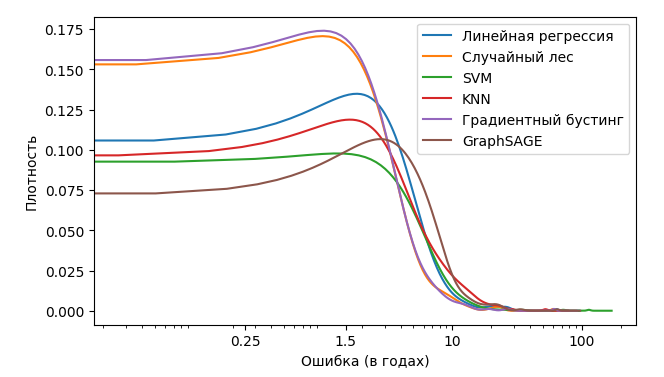
\includegraphics[width=\linewidth]{images/age_errors}

\caption{Плотность распределения ошибки для всех методов в задаче определения возраста}
\label{fig:age_errors}
\end{figure}

\clearpage